From our trained random forest regression model, we get a picture of the way
that redditors are. We get a glimpse of what useful, contributing redditors look
like, and what bad, non-contributing redditors look like.

On our test set of the data from about 3K redditors, we used our our regressive
model to get a reliability score $-1 \leq s_r \leq 1$. Then, we re-correlate
this score with input features to intuitively see what features are important or
not, and what features indicated useful and not-useful redditors.

\[ TODO \]

\begin{figure}[tb]
    \centering
    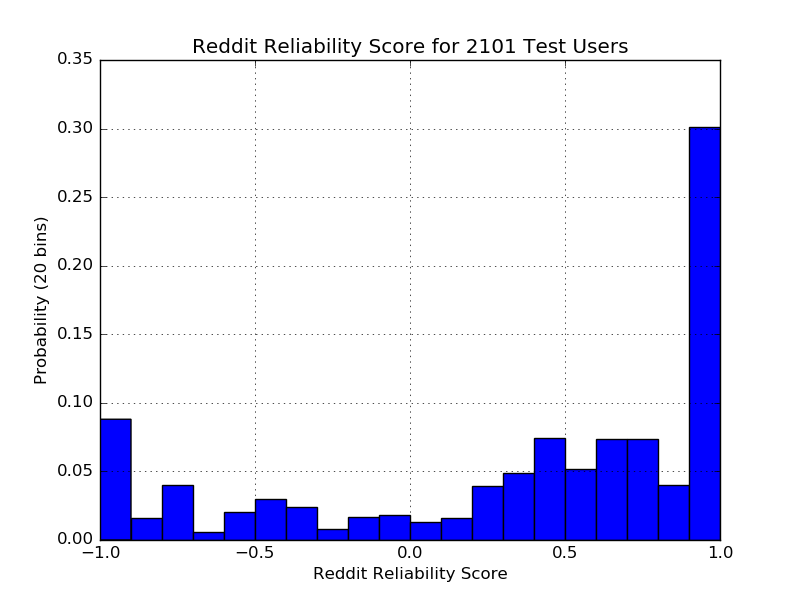
\includegraphics[width=\linewidth]{figures/data_20.png}
    \caption{The distribution of the reliability score $s_r$ of the sampled redditors, binned into twenty bins.}
    \label{fig:data_20}
\end{figure}

\begin{figure}[tb]
    \centering
    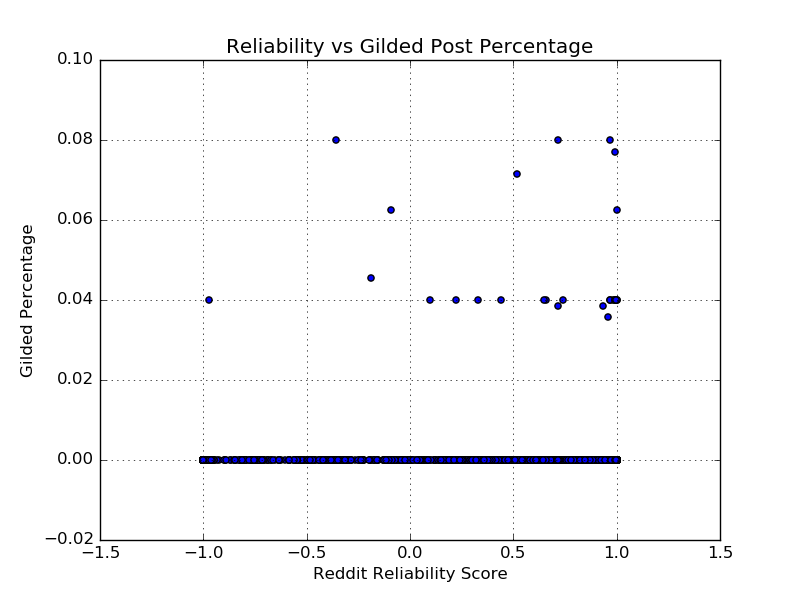
\includegraphics[width=\linewidth]{figures/reliability_gilded.png}
    \caption{The reliability score $s_r$ plotted against the percentage of gilded posts.}
    \label{fig:reliability_gilded}
\end{figure}

\begin{figure}[tb]
    \centering
    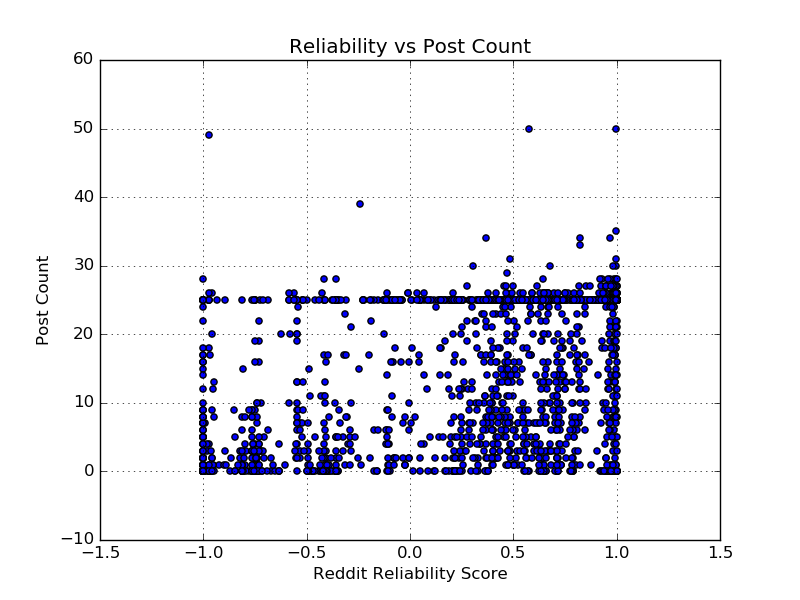
\includegraphics[width=\linewidth]{figures/reliability_post_count.png}
    \caption{The reliability score $s_r$ plotted against the number posts the redditor has made.}
    \label{fig:reliability_post_count}
\end{figure}

\begin{figure}[tb]
    \centering
    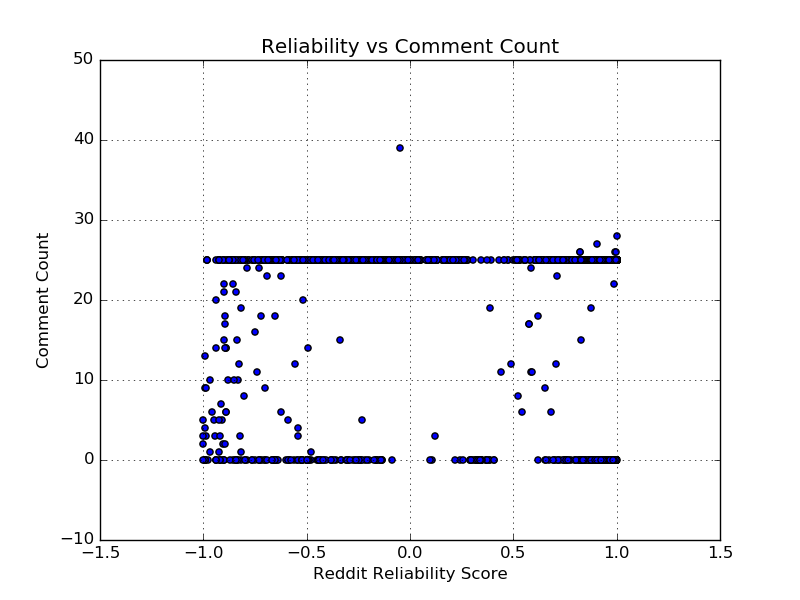
\includegraphics[width=\linewidth]{figures/reliability_comment_count.png}
    \caption{The reliability score $s_r$ plotted against the number posts the redditor has made.}
    \label{fig:reliability_comment_count}
\end{figure}

\begin{figure}[tb]
    \centering
    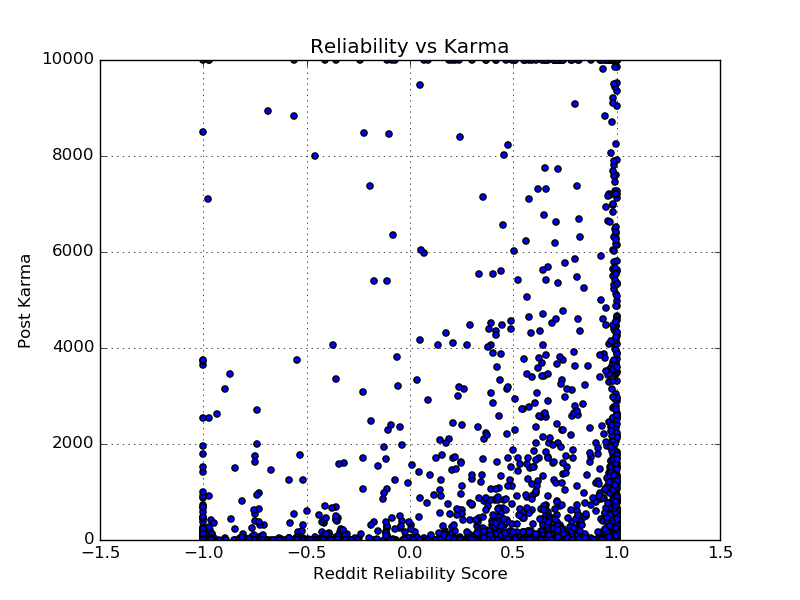
\includegraphics[width=\linewidth]{figures/reliability_post_karma.png}
    \caption{The reliability score $s_r$ plotted against the average Karma per post the redditor has made.}
    \label{fig:reliability_post_karma}
\end{figure}

\begin{figure}[tb]
    \centering
    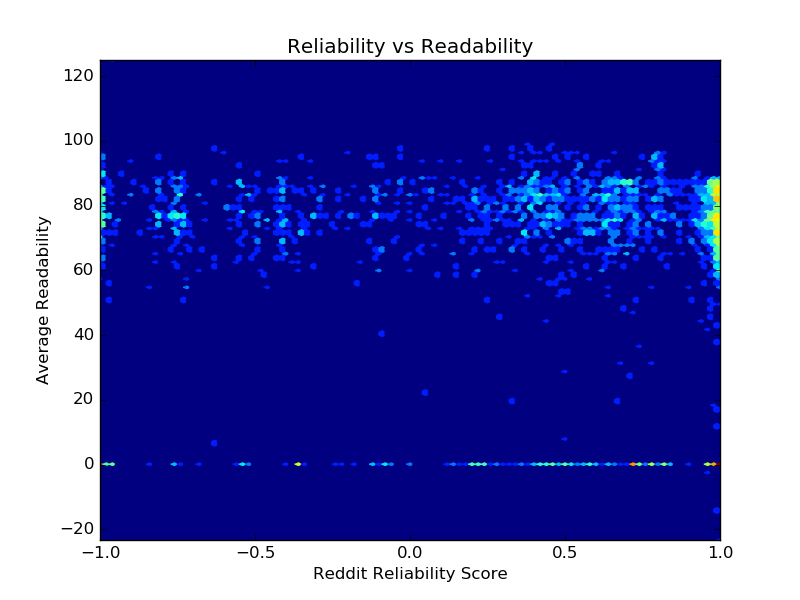
\includegraphics[width=\linewidth]{figures/reliability_readability.png}
    \caption{The reliability score $s_r$ plotted against the Flesch--Kincaid readability of their comments.}
    \label{fig:reliability_readability}
\end{figure}

\begin{figure}[tb]
    \centering
    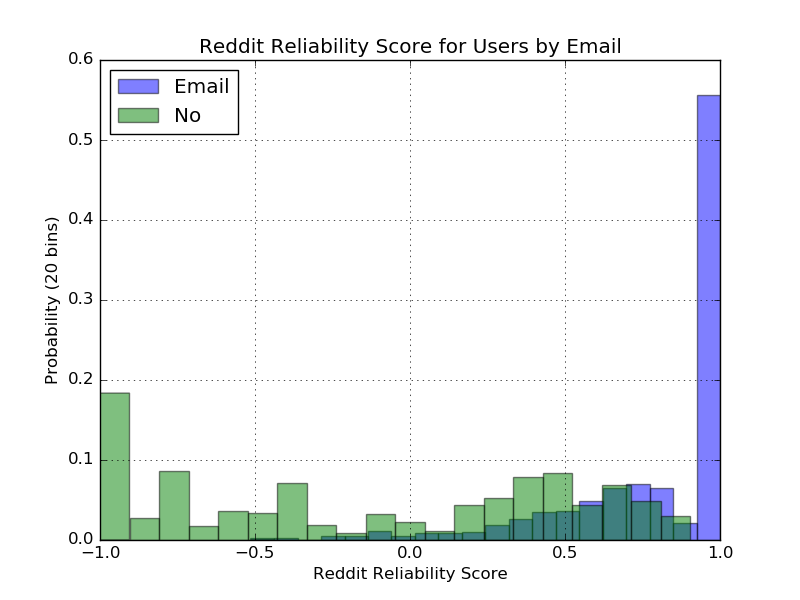
\includegraphics[width=\linewidth]{figures/data_20_email.png}
    \caption{The distribution of the reliability score $s_r$ of the sampled redditors, binned into twenty bins, separated by if they have a verified email address or not.}
    \label{fig:data_20_email}
\end{figure}
